\documentclass{report}
\usepackage[T1]{fontenc} % Fontes T1
\usepackage[utf8]{inputenc} % Input UTF8
\usepackage[backend=biber, style=ieee]{biblatex} % para usar bibliografia
\usepackage{csquotes}
\usepackage[portuguese]{babel} %Usar língua portuguesa
\usepackage{blindtext} % Gerar texto automaticamente
\usepackage[printonlyused]{acronym}
\usepackage{hyperref} % para autoref
\usepackage{graphicx}
\usepackage{indentfirst}
\usepackage{url}
\usepackage{textcomp}
\usepackage{pgfplots}
\usepackage{setspace} 

\bibliography{bibliografia}


\begin{document}
%%
% Definições
%
\def\titulo{Evolução dos Processadores}
\def\data{DATA}
\def\autores{António Caetano, Leonardo Luís}
\def\autorescontactos{(114094) antonio.caetano@ua.pt, (114093) leonardo.luis@ua.pt}
\def\versao{VERSAO}
\def\departamento{Dept. de Eletrónica, Telecomunicações e Informática}
\def\empresa{Universidade de Aveiro}
\def\logotipo{ua.pdf}
%
%%%%%% CAPA %%%%%%
%
\begin{titlepage}

\begin{center}
%
\vspace*{50mm}
%
{\Huge \titulo}\\ 
%
\vspace{10mm}
%
{\Large \empresa}\\
%
\vspace{10mm}
%
{\LARGE \autores}\\ 
%
\vspace{30mm}
%
\begin{figure}[h]
\center
\includegraphics{\logotipo}
\end{figure}
%
\vspace{30mm}
\end{center}
%
\begin{flushright}
\end{flushright}
\end{titlepage}

%%  Página de Título %%
\title{%
{\Huge\textbf{\titulo}}\\
{\Large \departamento\\ \empresa}
}
%
\author{%
    \autores \\
    \autorescontactos
}
%
\date{\today}
%
\maketitle

\pagenumbering{roman}

%%%%%% RESUMO %%%%%%
\begin{abstract}
O presente artigo analisa a evolução dos processadores ao longo da história, bem como as suas diferentes especificações, tendo em conta as necessidades de cada utilizador. De facto, existem diversos componentes diferentes, como o disco rígido, a placa-mãe, a \ac{RAM} e a \ac{GPU}, cada um com as suas determinadas funções. No entanto, o componente mais crucial num computador é sem dúvida a \ac{CPU}.

Desde os primórdios da era da computação, a unidade central de processamento (\ac{CPU}) sempre foi uma das atrações principais de qualquer novo dispositivo lançado para os consumidores. Tanto para os curiosos, como para um consumidor que deseja adquirir um processador adequado para um novo computador, é importante conhecer os diferentes tipos de \ac{CPU}s existentes no mercado. Desde o primordial Altair 8800, que possuía um \ac{Intel} 8080 com velocidade de 2MHz, até ao maior e mais recente iPhone 14 ou Samsung Galaxy Fold, a \ac{CPU} sempre foi o componente mais poderoso e essencial em qualquer dispositivo. Atualmente, escrevermos num teclado de um computador parece uma tarefa um tanto banal, mas como seria realmente a vida de cada um de nós se o revolucionário Charles Babbage não tivesse inventado o primeiro computador de uso geral?

Em pleno ano de 2022, estamos a chegar a um patamar onde a tecnologia alcançou um limite na sua vertente física. Deste modo, até que ponto os processadores irão continuar a evoluir de forma tão rápida como temos assistido até ao momento?

\end{abstract}




\tableofcontents
% \listoftables     % descomentar se necessário
% \listoffigures    % descomentar se necessário


%%%%%%%%%%%%%%%%%%%%%%%%%%%%%%%
\clearpage
\pagenumbering{arabic}

%%%%%%%%%%%%%%%%%%%%%%%%%%%%%%%%
\chapter{Introdução}
\label{chap.introducao}
Em pleno século XXI, a palavra “processador” é bastante conhecida pela maioria da população, no entanto, este termo é bastante confundido sem se saber realmente o que significa. A Unidade Central de Processamento, também conhecido como \ac{CPU}, é o principal componente de hardware de um sistema computacional. De facto, é o processador que é responsável na realização de instruções pelo utilizador, sendo capaz de executar operações aritméticas e lógicas de forma a executar determinados programas num computador. De um modo geral, podemos comparar este componente à função de um cérebro, que é capaz de processar inúmeras tarefas dentro de um sistema computacional.
Com a realização deste trabalho, espera-se dar a conhecer ao leitor a função e a importância da \ac{CPU}, os seus conceitos básicos, exemplos de grandes marcas de processadores e as suas diferenças quer positivas quer negativas, bem como a evolução histórica deste componente e o futuro dos processadores e microprocessadores.


\chapter{Conceitos básicos sobre um processador}
\label{chap.Conceitos básicos sobre um processador}
\section{O funcionamento geral de um processador}
Atualmente, todos os computadores modernos, smarthphones ou até mesmo smarthwatchs desempenham determinadas funções. Neste sentido, como é que será possível passarmos de uma simples calculadora para um videojogo num computador? De facto, o processador é o principal responsável no processamento de quase todos os comandos e operações realizados num computador, desde o controlo da memória \ac{RAM} do próprio computador até à execução de um programa \cite{Funcionamento1} (\ref{fig:Intel I9}).

\begin{figure}[h!]
\centering
  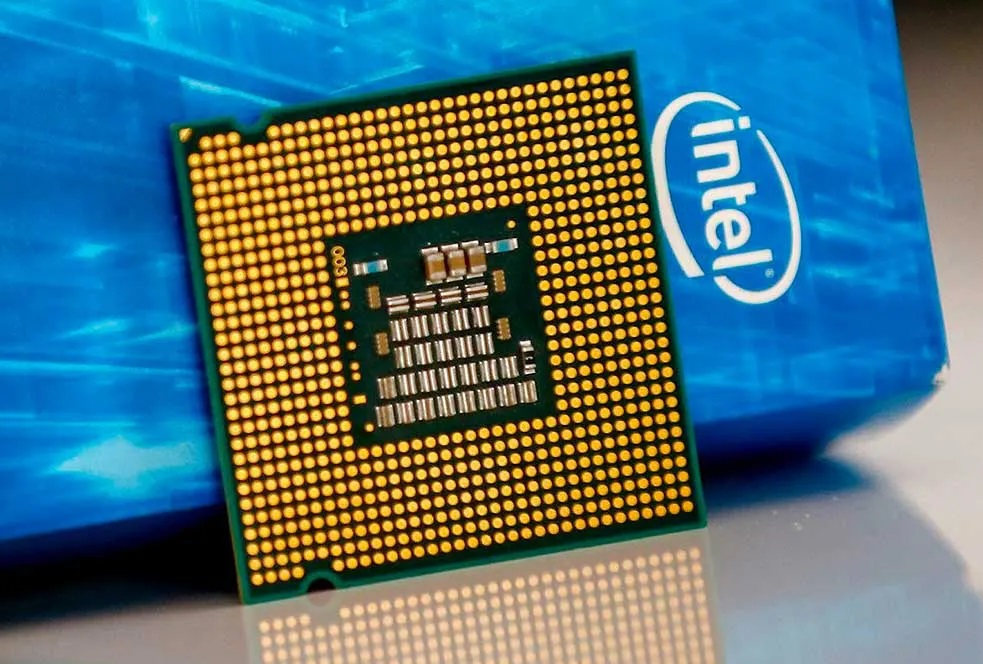
\includegraphics[width=1\textwidth]{relatorio latex/intel_chip_6.jpg}
  \caption{Um processador \ac{Intel} i9-10900k}
  \label{fig:Intel I9}
\end{figure}

Uma \ac{CPU} é composta basicamente pelos três seguintes tópicos: unidade lógica e aritmética (ULA), que executa operações lógicas e aritméticas; unidade de controlo (UC), que decodifica instruções, procura operações e tenta executá-las; e por fim os registradores que armazenam dados para o processamento\cite{Funcionamento5}.

Os novos processadores são construídos a partir de bilhões de transístores (\ref{fig:transístor1}), pequenos componentes que funcionam como interruptores ligados a uma corrente elétrica. Assim, as opções estar on ou off representam os números binários “1” e “0”, o “idioma dos computadores”. Neste âmbito, podem ser ligados e desligados diversas vezes por segundo, milhões (MHz) e até mesmo bilhões (GHz) de vezes por segundo. Desta forma, é a velocidade com que os transístores podem ser ligados e desligados num circuito que determina a velocidade final do relógio (frequência) deste chip. Este complexo processo é realizado a uma escala nanométrica, sendo fisicamente impossível observar este processo a olho nu\cite{Funcionamento4}.

\begin{figure}[h!]
\centering
  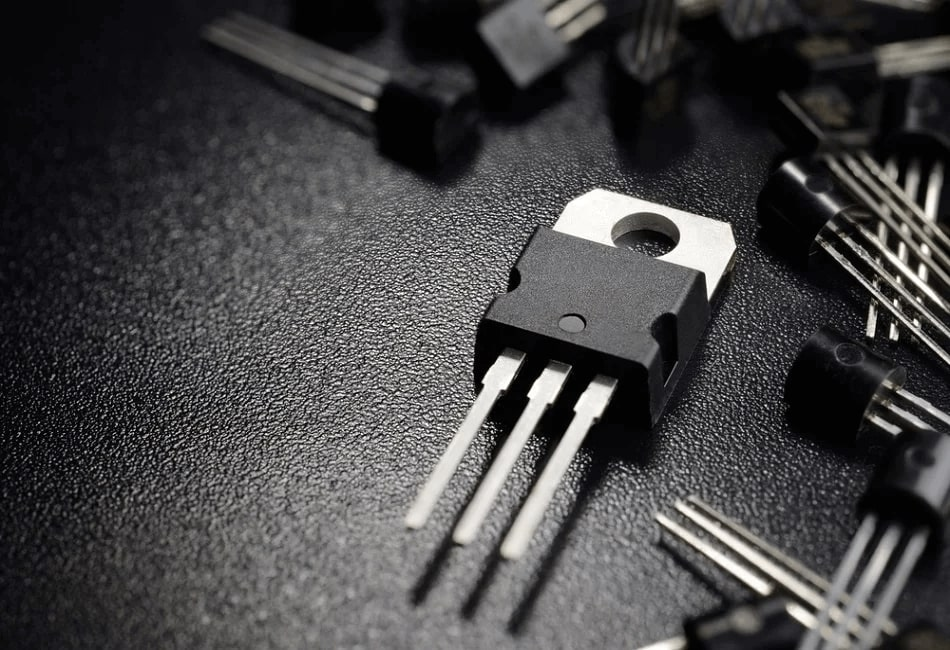
\includegraphics[width=1\textwidth]{relatorio latex/transistor.jpg}
  \caption{Um exemplo de um transístor}
  \label{fig:transístor1}
\end{figure}

 Por outro lado, os transístores podem ser dispostos de diversas formas, de modo a criar portões lógicos, que por sua vez, podem ser organizados para executar determinadas funções dentro de uma \ac{CPU}. Deste modo, o processador é o principal responsável em traduzir cada comando recebido pelo utilizador, gerando assim uma resposta, um output. Um dos objetivos principais na tecnologia da \ac{CPU} ao longo da história é tornar esses transístores cada vez menores, resultando num aumento e melhoria da velocidade do processador. Esta evolução irá ser desenvolvida mais à frente no presente artigo\cite{Funcionamento2}.
 
Na continuação da nossa abordagem, um processador recebe instruções de um programa e, posteriormente, realiza um determinado cálculo. Deste modo, este processo pode estar dividido em três categorias: busca, decodificação e execução. Estas operações só são possíveis devido a um conjunto de instruções predefinidas na memória \ac{RAM}, onde a\ac{CPU} irá procurar. De seguida, o processador decodifica a instrução e executa-a, usando importantes componentes dentro dele. A instrução ou cálculo executado pode envolver aritmética básica, comparando simplesmente números, ou movendo esses mesmos números dentro da memória, as possibilidades são infinitas\cite{Funcionamento3}!

É claro que o \ac{CPU} só funciona juntamente com outros hardwares incluídos num computador, estando este “chip de silício” localizado na placa principal do circuito, a placa-mãe (motherboard). O processador está separado da memória\ac{RAM} onde as informações são armazenadas temporariamente no computador, ao contrário de uma memória \ac{SSD}, por exemplo. Deste modo, o processador não consegue agir sozinho, estando sempre dependente dos outros componentes do computador, e vice-versa\cite{Funcionamento2}. 


\subsection{Arquitetura atual de um processador}

A arquitetura de um processador é um conjunto de instruções que descodificam e executam várias operações aritméticas e lógicas (\ac{ISA}).\cite{Arquitetura2}. Ao longo do tempo foram criadas diversos tipos de arquiteturas de processadores, como por exemplo, a \ac{CISC} e a \ac{RISC}(\ref{fig: RISC VS CISC}), bastante relevantes nos dias de hoje. 

Por um lado, a \ac{CISC}  é uma arquitetura que apresenta uma variedade extensa de linguagens de diferentes máquinas. O objetivo desta arquitetura é completar o seu trabalho em poucas linhas de código assembly, fazendo com que o compilador execute poucas tarefas para traduzir o código. Esta arquitetura é bastante conhecida devido ao x86 da \ac{Intel} e da \ac{AMD}\cite{Arquitetura2}.


Por outro lado, a \ac{RISC} foi desenvolvida de modo a melhorar o seu desempenho de uma forma relativamente simples, de onde provem o seu nome original - Reduced Instruction Set Computer. Dada esta característica, esta leva menos tempo a identificar determinadas instruções, tornando assim os resultados extremamente eficientes. Este tipo de arquitetura de processadores é muito importante na área dos videojogos, como por exemplo nas consolas Playstation 3, Xbox 360 e Nintendo. Com o evoluir da tecnologia, foram criados \ac{RISC} híbridos que, ao contrário dos antigos, conseguem aplicar uma correção nas instruções de comprimento de 16 bits com registradores de espaço 32 bits. Deste modo, os compiladores conseguem gerir melhor códigos \ac{RISC}\cite{Arquitetura2}.



\begin{figure}[h!]
\centering
  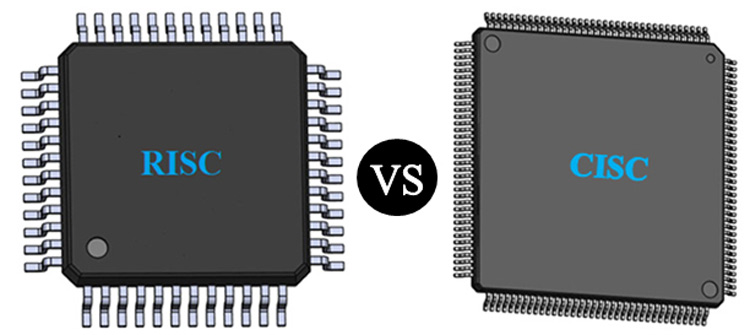
\includegraphics[width=1\textwidth]{relatorio latex/RISC.CISC.jpg}
  \caption{Arquitetura \ac{RISC} VS Arquitetura \ac{CISC}}
  \label{fig: RISC VS CISC}
\end{figure}



No entanto, estes tipos de arquitetura apresentam diversos defeitos. Por um lado, a \ac{CISC} consegue suportar mais instruções que a \ac{RISC}, mas esta apresenta menor velocidade. Já a \ac{RISC} não tem tanta capacidade para suportar um enorme número de instruções, quando comparado com a \ac{CISC}\cite{Arquitetura1}. 

Em suma, podemos concluir que a \ac{CISC} é a melhor das duas opções apresentadas. No entanto, nos dias de hoje, a \ac{CISC} optou por melhorar a sua arquitetura base, misturando o melhor dos dois mundos, arquitetura \ac{CISC} com arquitetura \ac{RISC}. Esta mistura é apenas capaz de processar instruções simples, dependendo sempre de instruções internas. Esta característica  é a responsável com que marcas de processadores tenham a sua própria assinatura\cite{Arquitetura1}.




\subsection{O desempenho de um processador}
O desempenho da \ac{CPU} de um computador é afetado por uma variedade de fatores. Atualmente, a maioria dos utilizadores desejam possuir computadores com componentes que funcionem com mais velocidade e apresentem melhor desempenho, especialmente, quando necessitam de realizar tarefas intensivas que peçam pela capacidade do processador. Este é um dos aspetos pelos quais as empresas continuam a aprimorar os seus processadores, de forma a possuírem um melhor desempenho em comparação com as suas versões anteriormente criadas. Por conseguinte, é importante perceber quais os principais fatores que podem afetar o desempenho do processador para saber quando pode ser necessário fazer um upgrade ao nosso hardware, neste caso, ao processador\cite{Desempenho2}.

As características de um processador estão diretamente ligadas à velocidade com que os seus programas vão ser executados num computador. De facto, existem diversos tipos de processadores no mercado, de 32 e 64 bits, com um ou mais núcleos, e compatíveis com diferentes motherboards, dependendo do tipo e da marca do processador escolhido. Embora existam processadores de 32 e 64 bits, as versões de 32 bits estão a cair em desuso, visto que os modelos de 64 bits permitem que a \ac{CPU} processe uma maior quantidade de dados, além de suportar mais memória \ac{RAM}. Enquanto os processadores de 32 bits não têm capacidade suficiente para possuir memória maior que 4 GigaBytes, os processadores de 64 bits suportam até 168 GigaBytes, um valor deveras avassalador. Já a quantidade de núcleos influencia diretamente a capacidade do processador em desempenhar multitarefas. Quanto maior for o número de núcleos, maior é a capacidade do computador em lidar com vários programas abertos ao mesmo tempo\cite{Desempenho1}.

Quanto aos processadores de um só núcleo, tal como o nome indica, podem apenas executar uma tarefa de cada vez, sendo os mais antigos no mercado. Como não permitem um bom desempenho no que toca a realizar diversas tarefas ao mesmo tempo, o computador fica cada vez mais lento à medida que se vão fornecendo novas instruções ao processador. Logo, para combater este problema, surgiram as \ac{CPU}s dual-core, que possibilitaram o dobro da eficácia de um processador, permitindo lidar com multitarefas de forma eficiente. Já os processadores quad-core são mais eficientes, uma vez que possuem quatro núcleos, possibilitando ao PC a execução de mais instruções sem sacrificar o seu próprio desempenho\cite{Desempenho1}. 

No que toca a processadores, a velocidade do clock é um tema bastante conhecido, mas na verdade o que é que significa? O clock é o número (GHz) que indica efetivamente quantas instruções por segundo uma \ac{CPU} é capaz de processar, no entanto, não é só isto que afeta o desempenho deste chip. A velocidade do clock é igualmente importante quando se compara \ac{CPU}s da mesma marca ou geração de produtos (\ref{fig:Intel Clock}). Assim, quando os componentes são iguais, uma maior velocidade de clock propicia um processador mais rápido. Todavia, é de notar que um processador de 3 GHz em 2010 apresenta um menor rendimento quando comparado a um processador de 2 GHz em 2020\cite{Desempenho2}.

\begin{figure}[h!]
\centering
  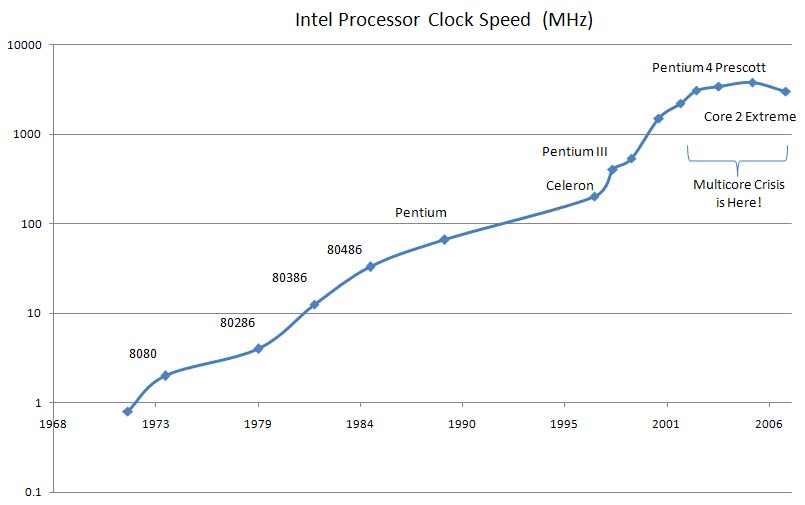
\includegraphics[width=1\textwidth]{relatorio latex/clockspeeds.jpg}
  \caption{Velocidade de clock de processadores da Intel ao longo do tempo}
  \label{fig:Intel Clock}
\end{figure}


Por seu turno, um cache é uma memória de alta velocidade junto ou relativamente perto de um processador, sendo utilizado para armazenar instruções e os dados mais usados pelo utilizador. Ao executar programas, um sistema de computador está constantemente a trocar de dados, de dentro para fora da memória cache e da \ac{RAM}. Quando um conjunto de instruções é frequentemente utilizado é ineficiente, em termos de desempenho, para uma \ac{CPU} ir buscá-los a partir da memória \ac{RAM} cada vez que os utiliza. Para resolver este problema, existe a memória cache que é então usada para armazenar as instruções que provavelmente irão ser utilizadas. Tal como acontece com a \ac{RAM}, a memória cache é apagada quando o computador se desliga\cite{Desempenho2}.


\section{Aplicações atuais}
Com tanta escolha e variedade de \ac{CPU}s, é importante saber quais as principais aplicações de um processador para determinar qual a melhor escolha para as necessidades de cada utilizador. O propósito de um processador é fazer a computação real de um computador, o que inclui gerir a memória, manipular a entrada dos usuários, enviar saídas (outputs) e fazer os diferentes cálculos aritméticos necessários\cite{Aplicações1/Velocidade1}.

Atualmente, o processador não é tão importante para o desempenho geral de um sistema computacional quando comparado com alguns anos atrás. No entanto, é verdade que sem ele é impossível executar qualquer operação ou executar qualquer software. Assim, ainda tem um papel fundamental na resposta e velocidade do processamento de instruções num computador. De facto, os jogadores de videojogos (gamers) encontram um benefício extra em possuir velocidades mais altas do clock por parte da \ac{CPU}, tal como editores de vídeos e de imagens, pois terão uma melhoria significativa em relação a um aumento do número de núcleos da \ac{CPU}. É importante salientar que também é necessário ter \ac{RAM} suficiente e armazenamento rápido (disco \ac{SSD}) que irá processar os dados para a \ac{CPU}\cite{Aplicações1/Velocidade1}.

Em suma, podemos encontrar uma \ac{CPU} em praticamente todos os dispositivos eletrónicos. Ou seja, qualquer equipamento tecnológico que se qualifique como um computador, que é uma sistema que recebe entradas (inputs), processa-as e retorna-as como saídas (outputs), contém um processador. Exemplos disso são, por exemplo, um computador portátil, uma televisão inteligente, um smartphone ou um tablet, entre outros\cite{Aplicações1/Velocidade1}.





\chapter{Evolução da CPU}
\label{chap.Evolução da CPU}
\section{História e criação dos processadores}

Ao longo dos tempos, os processadores foram evoluindo progressivamente, criando um avanço enorme na tecnologia existente. A evolução do processador ocorre desde os tempos antigos, tal como a primeira calculadora mecânica criada pelo matemático e físico Blaise Pascal, ou como o inesquecível computador \ac{ENIAC}, o primeiro a ser criado\cite{Historia1}(\ref{fig:ENIAC}). 


\begin{figure}[h!]
\centering
  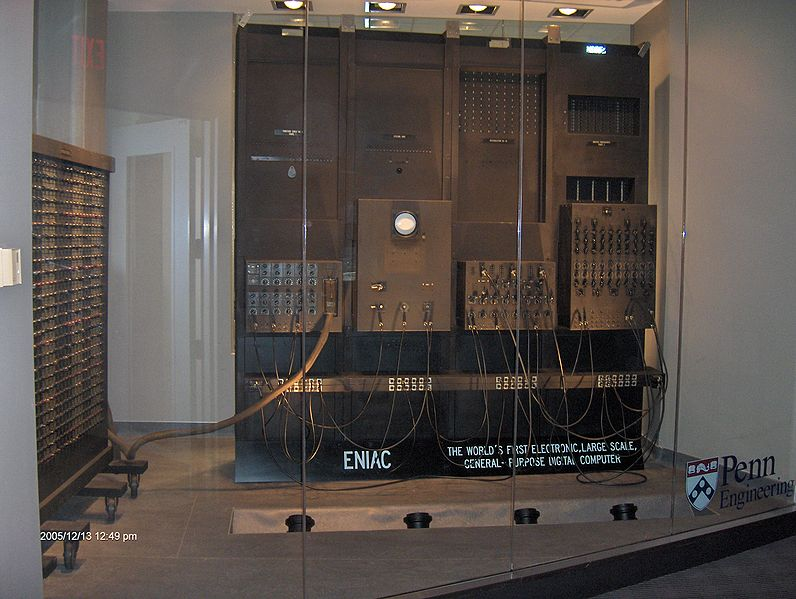
\includegraphics[width=1\textwidth]{relatorio latex/ENIAC_Penn1.jpg}
  \caption{O primeiro computador do mundo (\ac{ENIAC})}
  \label{fig:ENIAC}
\end{figure}

Existem várias referências a um processador nos tempos antigos, no entanto, este só começou a ser popular em 1971, quando Frederico Faggin criou o primeiro microprocessador denominado \ac{Intel} 4004 \cite{IntelH}. Este processador possuía apenas 4 bits, com capacidade de 640 bytes, uma capacidade surpreendente para o ano de 1971, onde se realizavam meras operações aritméticas. Esta \ac{CPU} era constituída por 2300 transístores para processar 60000 instruções por segundo, sendo usado para cálculos pouco complexos (4 operações), com a vantagem de possuir um tamanho reduzido, levando a um menor custo de energia\cite{Historia1}.

No ano seguinte, em 1972, foi criado o \ac{Intel} 8008. Este processador era uma versão melhorada do seu antecessor\cite{IntelH}. De facto, este novo chip foi o primeiro a ter 8 bits, contendo uma capacidade de memória de 16 Kbytes.
Já em 1974, foi lançado o \ac{Intel} 8080 com um desempenho ainda maior, possuindo com um clock de 2MHz, sendo capaz de executar um programa lançado pela Microsoft, o "Basic". Apesar de apresentar a mesma capacidade que o processador anterior, este possuía 4 Kbytes de memória \ac{RAM}\cite{Historia1} . 
Em 1979 foi desenvolvido o primeiro processador da \ac{Intel} para \ac{PC}, o \ac{Intel} 8086. esta novidade continha 16 bits com um barramento de dados internos e externos. Quando foi lançado, a maioria dos dispositivos eram de 8 bits, pelo que não teve muito sucesso, dado que, modificar os dispositivos, apresentava um custo elevado por parte dos utilizadores\cite{Historia1}.

Foi no ano de 1982 que os processadores ganharam outro rumo, iniciando assim a segunda geração de processadores com o lançamento do I80286, um processador criado pela \ac{Intel}\cite{IntelH}. 



















Uma das características deste processador foi a capacidade de utilizar até 16 Mb e possuir um hardware com tecnologia multitasking. Devido a esta tecnologia foi possível com que sejam executados programas em intervalos, intercalando de um para outro\cite{Historia1}. Nesse próprio ano surgiu uma nova empresa, a \ac{AMD}. Nesse ano, esta empresa apresentou um processador denominado de 286A, bastante semelhante com o 286 da \ac{Intel}\cite{deevoluccao}.

Em 1985, a \ac{Intel} lançou o processador I80386, onde a terceira geração começou. Este foi o primeiro processador com totalmente 32 bits, ou seja, ele fazia tanto o processo interno como o externo a 32 bits. Foi a partir deste que o conjunto de instruções padrão x86 se começaram a formar. Quanto às capacidades, estas também tiveram uma mudança, podendo manipular 4 Gb de memória\cite{Historia1}. Nesse ano a sua empresa rival atual, a \ac{AMD}, criou um processador, o Am386. Este era praticamente igual ao anterior criado, com apenas algumas melhorias e modificações. A \ac{AMD} fez duas versões deste processador, uma com suporte de 32 bits e outra com o suporte de 16 bits\cite{deevoluccao}.


Em 1992, foi lançada a gama Pentium(\ref{fig:Pentium} )também conhecida por P54C. Este novo processador era constituído por vários clocks internos diferentes, tendo chegado a 200 MHz. Quanto às suas especificações este processador continha 3,1 milhões de transístores, com um cache interno e 16Kb (8Kb para a extração e outros 8Kb para dados). Nos três anos seguintes, com o sucesso do processador Pentium, a \ac{AMD} tentou produzir um processador de mesmo calibre, o 586, porém não foi bem acolhido pelos consumidores. Com o passar do tempo a gama Pentium foi evoluindo, tendo criado vários outros processadores, tal como a sua rival \ac{AMD}\cite{Historia1}\cite{deevoluccao}.

\begin{figure}[h!]
\centering
  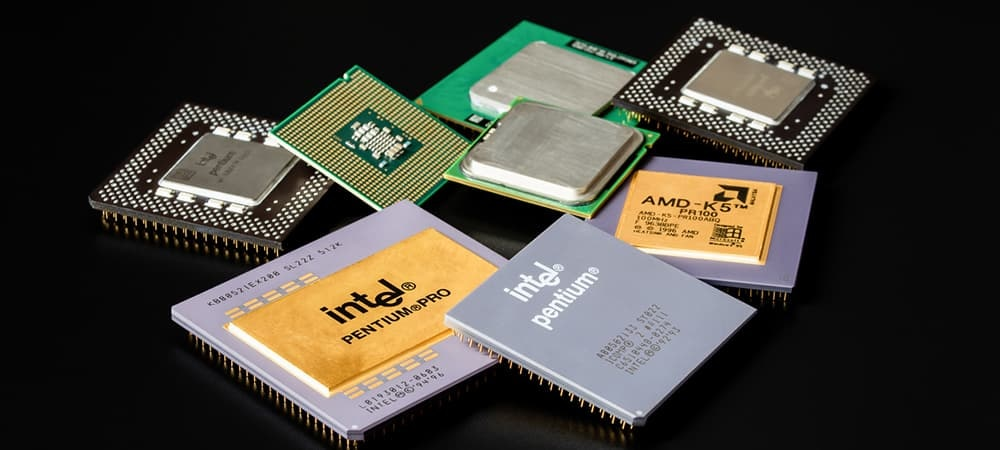
\includegraphics[width=1\textwidth]{relatorio latex/Pentium.jpg}
  \caption{Família de Processadores Pentium}
  \label{fig:Pentium}
\end{figure}




Em 2006 a \ac{Intel} criou mais um processador: o \ac{Intel} Itinium. Este processador apresentava um dual core, com uma elevada eficácia, tendo a capacidade de executar aplicações de 32 e de 64 bits, uma novidade para o ano de 2006. Este processador apresentava uma mistura de arquitetura \ac{CISC} e \ac{RISC}, possuindo velocidades ainda mais rápidas\cite{Historia1}. 

Nos dias de hoje, os processadores mais utilizados pelos consumidores são os da gama \ac{Intel} Core e os \ac{AMD} Ryzen. As características desta linha de \ac{CPU}s irão ser retomadas e abordadas mais à frente.

 
\section{Poder e velocidade de um processador na atualidade}
Como já mencionado anteriormente, a velocidade do clock é a forma mais comum de medir a velocidade de um processador. É assim medida em Hertz, que é o número de vezes por segundo que a tensão elétrica no processador alterna entre baixa e alta. Desta forma, o processador utiliza essas oscilações criadas para realizar os cálculos de forma física\cite{Aplicações1/Velocidade1}. 

Mais concretamente, os processadores são unidades dual ou quad-core. Isto significa que estão configurados para funcionar como se fossem dois ou quatro processadores separados. Por outras palavras, um sistema computacional, dual ou quad-core, pode trabalhar de forma mais eficiente dado que consegue atribuir um ou mais núcleos a cada tarefa específica. Além disso, a velocidade do clock refere-se ao processador como um todo, sendo executado nessa determinada velocidade, independentemente de como os núcleos são atribuídos a cada determinada tarefa\cite{Velocidade2}.

Por outro lado, o conhecido termo overclocking envolve modificar um computador de forma a que um processador seja executado a uma velocidade de clock não recomendada, ou seja, mais rápida do que sua configuração padrão. Esta é uma tarefa complicada e bastante arriscada para quem não está bem informado sobre o hardware de um computador, podendo levar a problemas e bugs no sistema. Pode-se concluir que o overclocking aumenta significamente o consumo de energia e aumenta o risco de aquecimento elevado que poderá causar danos irreparáveis na \ac{CPU}\cite{Velocidade3}.

De facto, vivemos num mundo onde a tecnologia muda drasticamente de ano para ano, não sendo exceção para os processadores. Atualmente, em pleno ano 2022, os dois processadores premium mais rápidos que dominam o mercado são o \ac{Intel} Core i9-12900K e o seu concorrente \ac{AMD} Ryzen 9 5900X(\ref{fig:I9 Ryzen9}). Relativamente às marcas e diferentes tipos de processadores, iremos abordar este assunto no tópico seguinte.

\begin{figure}[h!]
\centering
  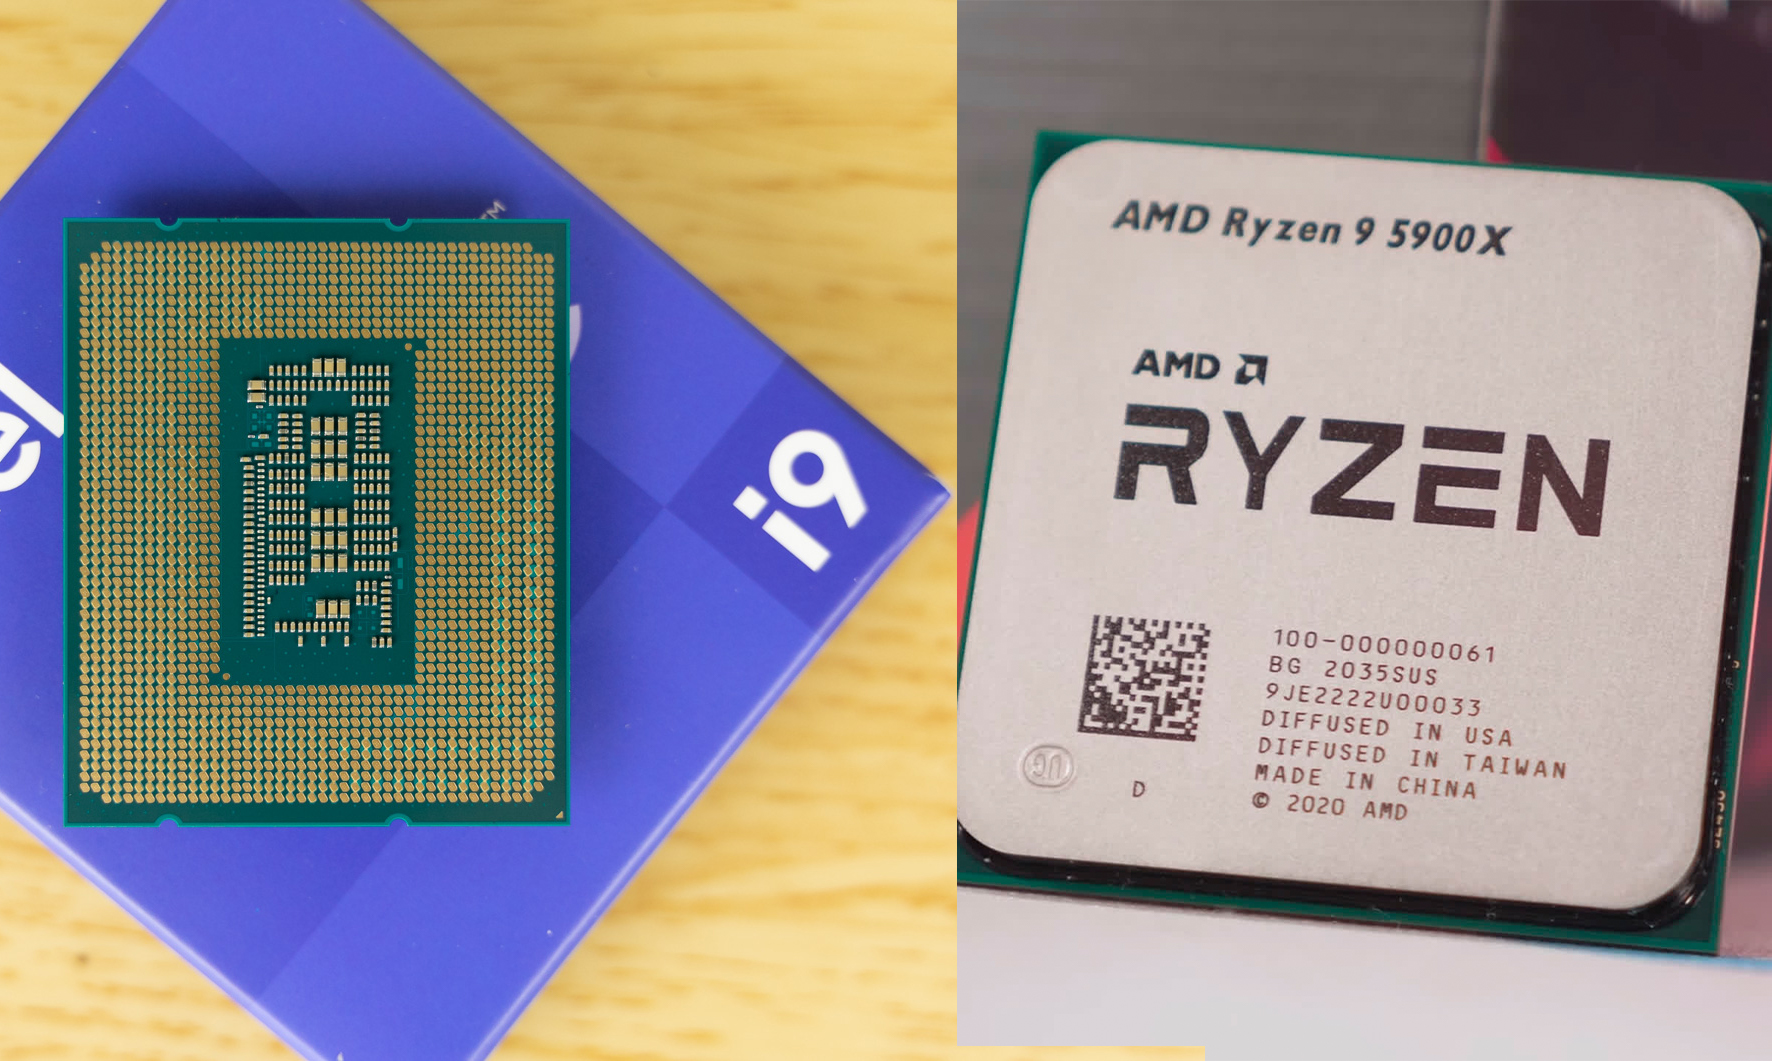
\includegraphics[width=1\textwidth]{relatorio latex/I9 & Ryzen 9.jpg}
  \caption{Exemplo do processador \ac{Intel} Core i9-12900K e \ac{AMD} Ryzen 9 5900X}
  \label{fig:I9 Ryzen9}
\end{figure}


De um modo geral, velocidades mais rápidas do clock do processador aumentará diretamente a rapidez das tarefas num computador, tornando melhor a experiência do utilizador e reduzindo assim o tempo de espera para interagir, como por exemplo, com aplicações de um sistema operativo.




\chapter{Diferenças entre processadores}
\label{chap.Diferenças entre processadores}
\section{Diferentes tipos de processadores}

Existem inúmeros tipos de modelos e marcas de processadores disponíveis, com características e potências diferentes. Com efeito, é primordial conhecer qual o tipo de processador adequado a cada utilizador. Dependendo das preferências de cada utilizador, um determinado processador será mais ou menos adequado do que o outro. Na realidade, não existem \ac{CPU}s melhores ou piores, mas modelos mais adequados a determinadas funções\cite{Diferentes1}. 
Existem inúmeros processadores no mercado, no entanto, iremos apenas abordar os principais e os mais funcionais para cada utilizador. Atualmente, em termos de smarthphones, o A15 Bionic é o processador mais rápido da Apple e o Qualcomm Snapdragon 8 Plus Gen 1 o mais rápido nos Androids (\ref{fig:SP CPUs})\cite{Diferentes3}. Enquanto o primeiro contém 6 núcleos e 15 bilhões de transístores, nos rivais Androids, este processador apresenta uma arquitetura de 64 bits, uma velocidade de clock de até 3.2 GHz e 8 núcleos. Comparando com alguns anos atrás, podemos constatar que são valores absurdos quando falamos de meros smarthphones\cite{AppleA15}\cite{Snapdragon8}.

\begin{figure}[h!]
\centering
  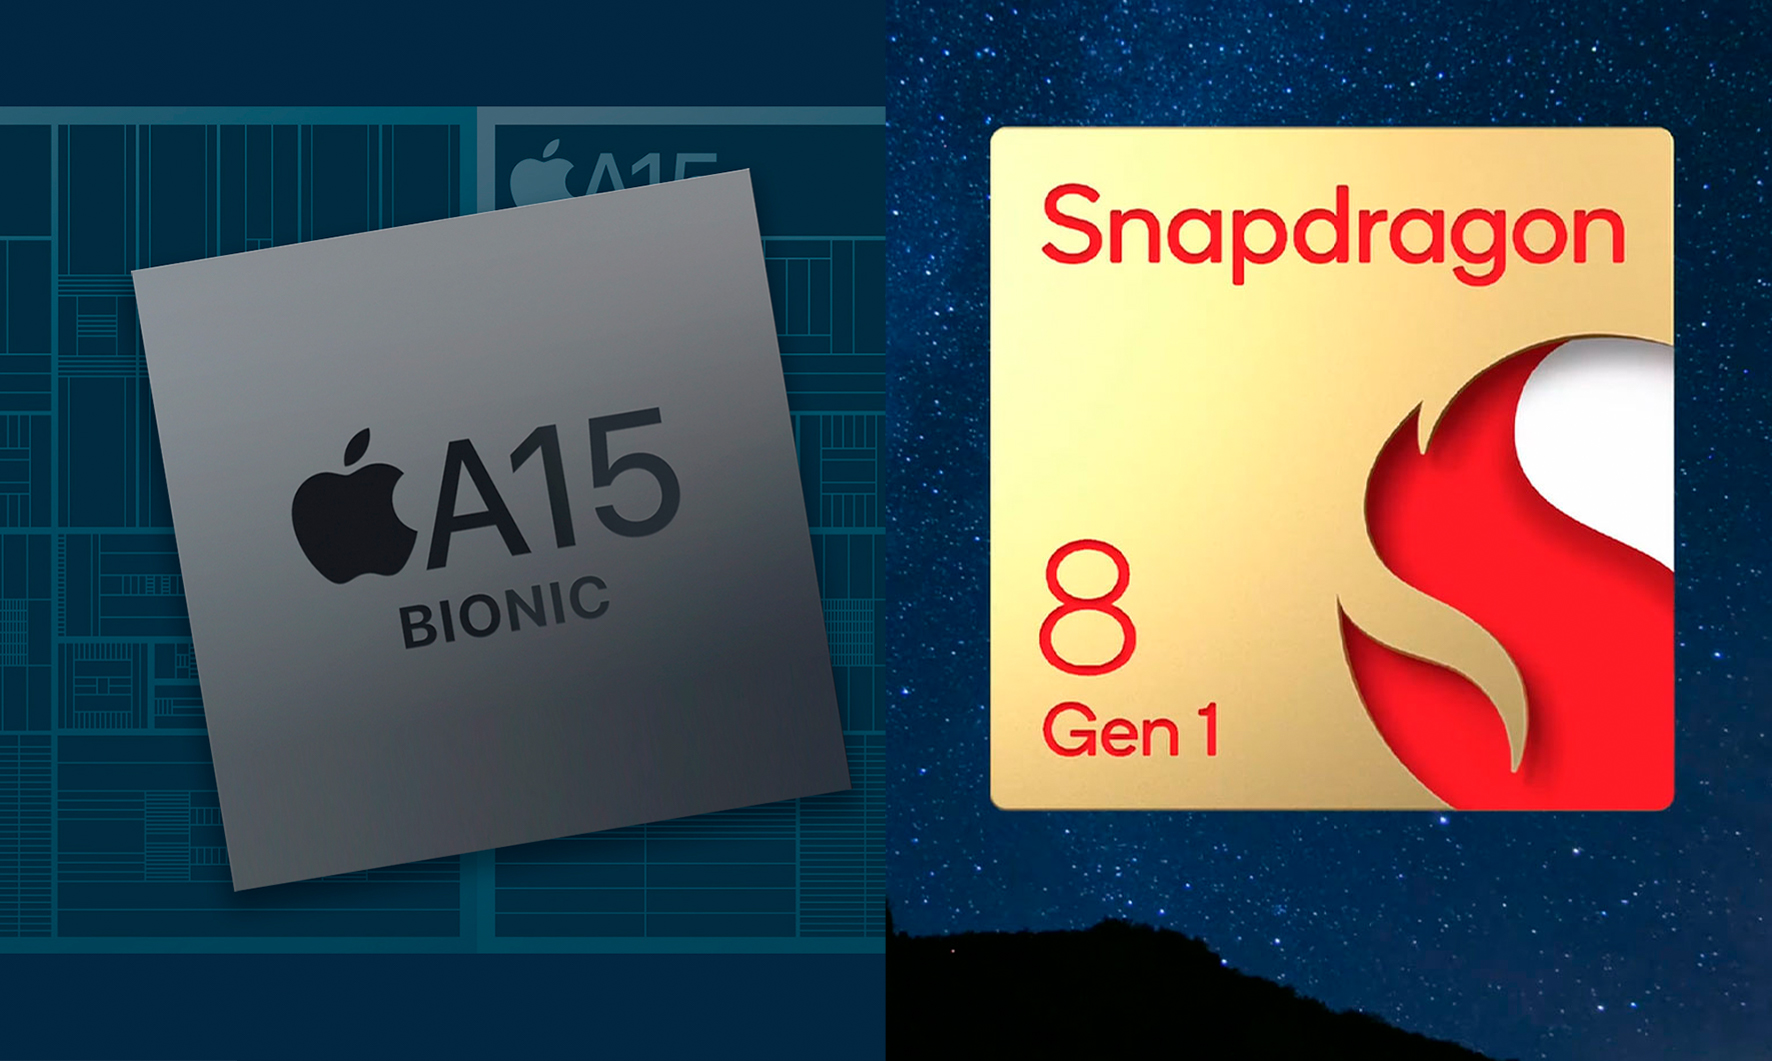
\includegraphics[width=1\textwidth]{relatorio latex/smathphones cpus.jpg}
  \caption{Exemplo do processador A15 Bionic e do Snapdragon 8 Plus Gen 1}
  \label{fig:SP CPUs}
\end{figure}

Por outro lado, nos computadores - apesar de começarem a surgir novas marcas de processadores como o Exynos da Samsung - a \ac{Intel} e a \ac{AMD} dominaram totalmente o mercado. Neste domínio, a \ac{Intel} sempre foi a mais popular e está presente no mercado como a principal marca de processadores, devido à sua versatilidade e compatibilidade com diferentes placas mãe. Existem diferentes modelos, alguns mais baratos e com menos performance, e outros com um preço mais elevado para quem tem a necessidade de obter um maior desempenho. Deste modo, dentro da linha \ac{Intel}, existe a seguinte série de processadores: \ac{Intel} Core; \ac{Intel} Pentium; \ac{Intel} Celeron; \ac{Intel} Xeon; \ac{Intel} Xeon Phi; \ac{Intel} Itanium; \ac{Intel} Atom e \ac{Intel} Quark SoC\cite{Diferentes2}. A linha mais popular desta marca é a \ac{Intel} Core, dado que apresenta processadores para todo o tipo de carteira e em função das necessidades de cada utilizador. Assim, dentro desta linha, foi desenvolvido o  I3 para as tarefas do dia a dia, apresentando, por sua vez, um vantagem em termos de custo-benefício. De seguida, surge o I5 que é um processador de alto desempenho, que pode ter 2 ou 4 núcleos. Já com um maior custo, chega o I7, cujo principal foco é fornecer alta velocidade e um desempenho máximo, com 6 a 10 núcleos, apresentando tecnologias de hyperthreading e TurboBoost. Por fim, o I9 apresenta processadores para workstations mais poderosas da \ac{Intel}, voltado nomeadamente para profissionais da área de engenharia e arquitetura que necessitam de qualidade e eficiência nos seus projetos. Esta linha contém, para além de todas as tecnologias anteriormente mencionadas, de 10 a 18 núcleos e 36 threads respetivamente, tendo a capacidade para trabalhar com conteúdo de 4K com alto desempenho \cite{Diferentes2}.

Por outro lado, a \ac{AMD} , concorrente direta da \ac{Intel}, é uma empresa norte americana também especializada em processadores. Com efeito, esta empresa possui um leque de processadores distintos, cada um criado para determinado tipo de tarefas e desempenho. Assim, existem 6 grandes categorias de \ac{CPU}s da \ac{AMD}: \ac{AMD} Ryzen; \ac{AMD} Ryzen PRO; \ac{AMD} Ryzen Threadripper; \ac{AMD} A-Series; \ac{AMD} FX; \ac{AMD} A-Series PRO. Dentro destas categorias, a que possui mais destaque é sem dúvida a \ac{AMD} Ryzen pelo seu desempenho superior. Além disso, disponibiliza processadores que podem ir até 16 núcleos. Esta linha apresenta 3 categorias de processadores: a saber Ryzen 3,5 e 7, cada um deles com um determinado uso específico\cite{Diferentes2}.





\chapter{Lei de Moore}
\label{chap.Lei de Moore}
A lei de Moore - que no fundo é somente uma observação feita pelo engenheiro Gordon E. Moore, cofundador da Intel -, demonstra que "o número de transístores num circuito integrado a cada dois anos duplica o seu valor". De um modo geral, esta observação demonstra que, ao longo do tempo, é possível aumentar o número de transístores, com um custo mínimo e com a mesma quantidade de espaço utilizado. Como supramencionado anteriormente, um maior número de transístores equivale a um processador mais rápido e eficiente. A velocidade da \ac{CPU} tem sido historicamente medida por “Instruções por segundo”. Na atualidade, os novos processadores são tão rápidos que podem ser medidos em bilhões de instruções por segundo. O gráfico  representado a seguir, \ref{[5.1]}, demonstra como as velocidades do processador aumentaram significamente com o decorrer do tempo, como comprova a Lei de Moore\cite{Lei1}.


\begin{figure}[h!]
\centering
  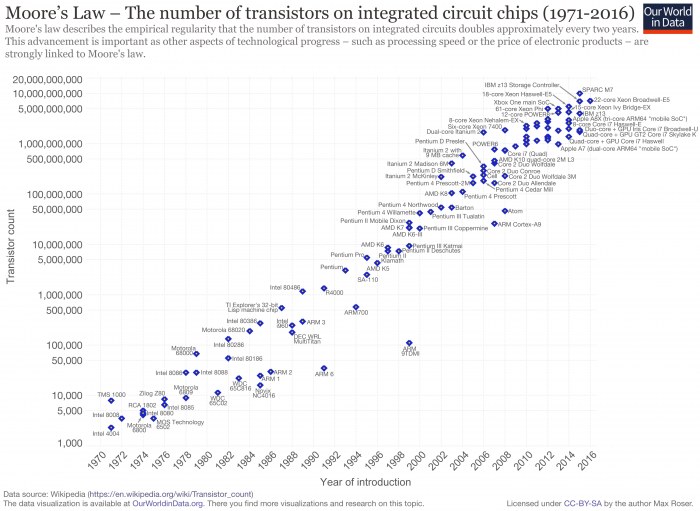
\includegraphics[width=1\textwidth]{relatorio latex/graph1.png}
  \caption{O gráfico mostra o aumento no número de transístores em processadores, de 1971 a 2016}
  \label{fig:graph1}
\end{figure}

\begin{tikzpicture}
\begin{axis}  
[  
    title={Lei de Moore },
    ybar,  
    enlargelimits=0.15,  
    ylabel={Número de Transístores (em milhares)},  
    xlabel={Ano},  
    symbolic x coords={1975, 1985, 1995, 2005},  
    xtick=data,  
     nodes near coords, 
    nodes near coords align={vertical},  
    ]  
\addplot coordinates {(1975,10) (1985,1000) (1995,10000) (2005,1000000) };  

  \label{[5.1]}
\end{axis}  
\end{tikzpicture}  



Como podemos verificar na figura \ref{fig:graph1}, o aumento significativo de desempenho dos processadores está a estabilizar, visto que, com o avanço tão rápido da tecnologia, é cada vez mais difícil existir picos tão elevados em termos de desempenho e eficiência tecnológica. Mais, podemos deduzir que estamos a chegar a um ponto onde é cada vez mais difícil agrupar transístores devido aos limites da Física\cite{Lei1}\cite{Lei2}.

Em suma, verificamos que estamos a chegar ao fim da Lei de Moore, não só pelos limites da Física como também pelo facto de que está a ser desenvolvido sistemas que exigem menos recursos por parte da \ac{CPU}. Além disso, o custo para pesquisas de novos e melhores processadores estão cada vez mais caros, ao que acresce o consumo de energia provocado pelo aumento da eficiência e velocidade dos processadores\cite{Lei2}.


\chapter{O futuro dos microprocessadores}
\label{chap.O futuro dos microprocessadores}

A tecnologia, nos dias de hoje, tem evoluído de forma significativa, designadamente na área dos processadores. Com efeito, este tipo de desenvolvimento está intimamente ligado à criação de diversos processadores com alto desempenho. 


\cite{Blog2} . 
\begin{figure}[h!]
\centering
  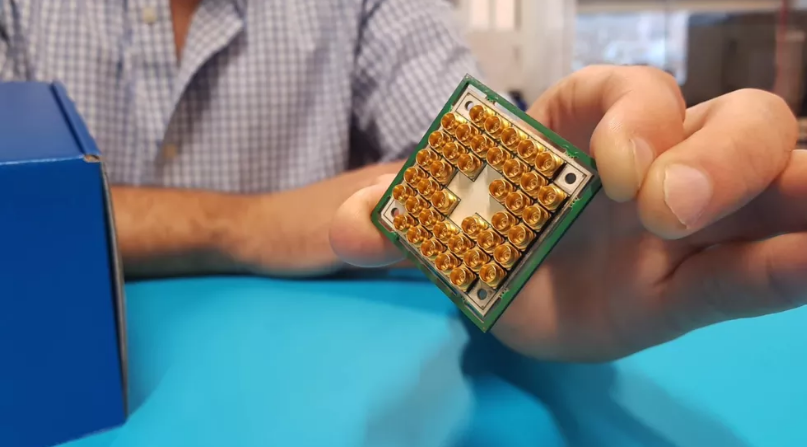
\includegraphics[width=1\textwidth]{relatorio latex/cpu quantico.PNG}
  \caption{Exemplo de um processador quântico desenvolvido pela \ac{Intel}}
  \label{fig:cpu_q}
\end{figure}


Prevê-se que o ano 2030 venha a ser o ano em que se atinge  o expoente máximo na área dos processadores e dos seus respetivos desempenhos. Por outras palavras, estas \ac{CPU}s irão ser constituídas por 50 bilhões de transístores, o que irá possibilitar uma velocidade de topo \cite{Blog2}.
Outro marco previsto nesse ano está relacionado com a criação de processadores quânticos que serão disponibilizados no mercado. Esta será, sem dúvida, um ponto de viragem na história dos processadores\cite{Blog1}.

De facto, estes processadores quânticos(\ref{fig:Quantico}) apresentam uma diferença significativa em relação aos processadores eletrónicos, visto que  operam em qubits (quantum bits). Desta forma, devido à natureza da física quântica, antes de se proceder à leitura do bit quântico, o seu estado pode ser diferente de 0 ou 1, ou seja, consegue estar na interseção entre estes dois estados, diferentemente de um processador regular. Devido a este processo, a \ac{CPU} terá a capacidade de fazer os mesmos cálculos mas em velocidades muito superiores à que estamos familiarizados(\ref{fig:cpu_q})\cite{Blog1}.
\begin{figure}[h!]
\centering
  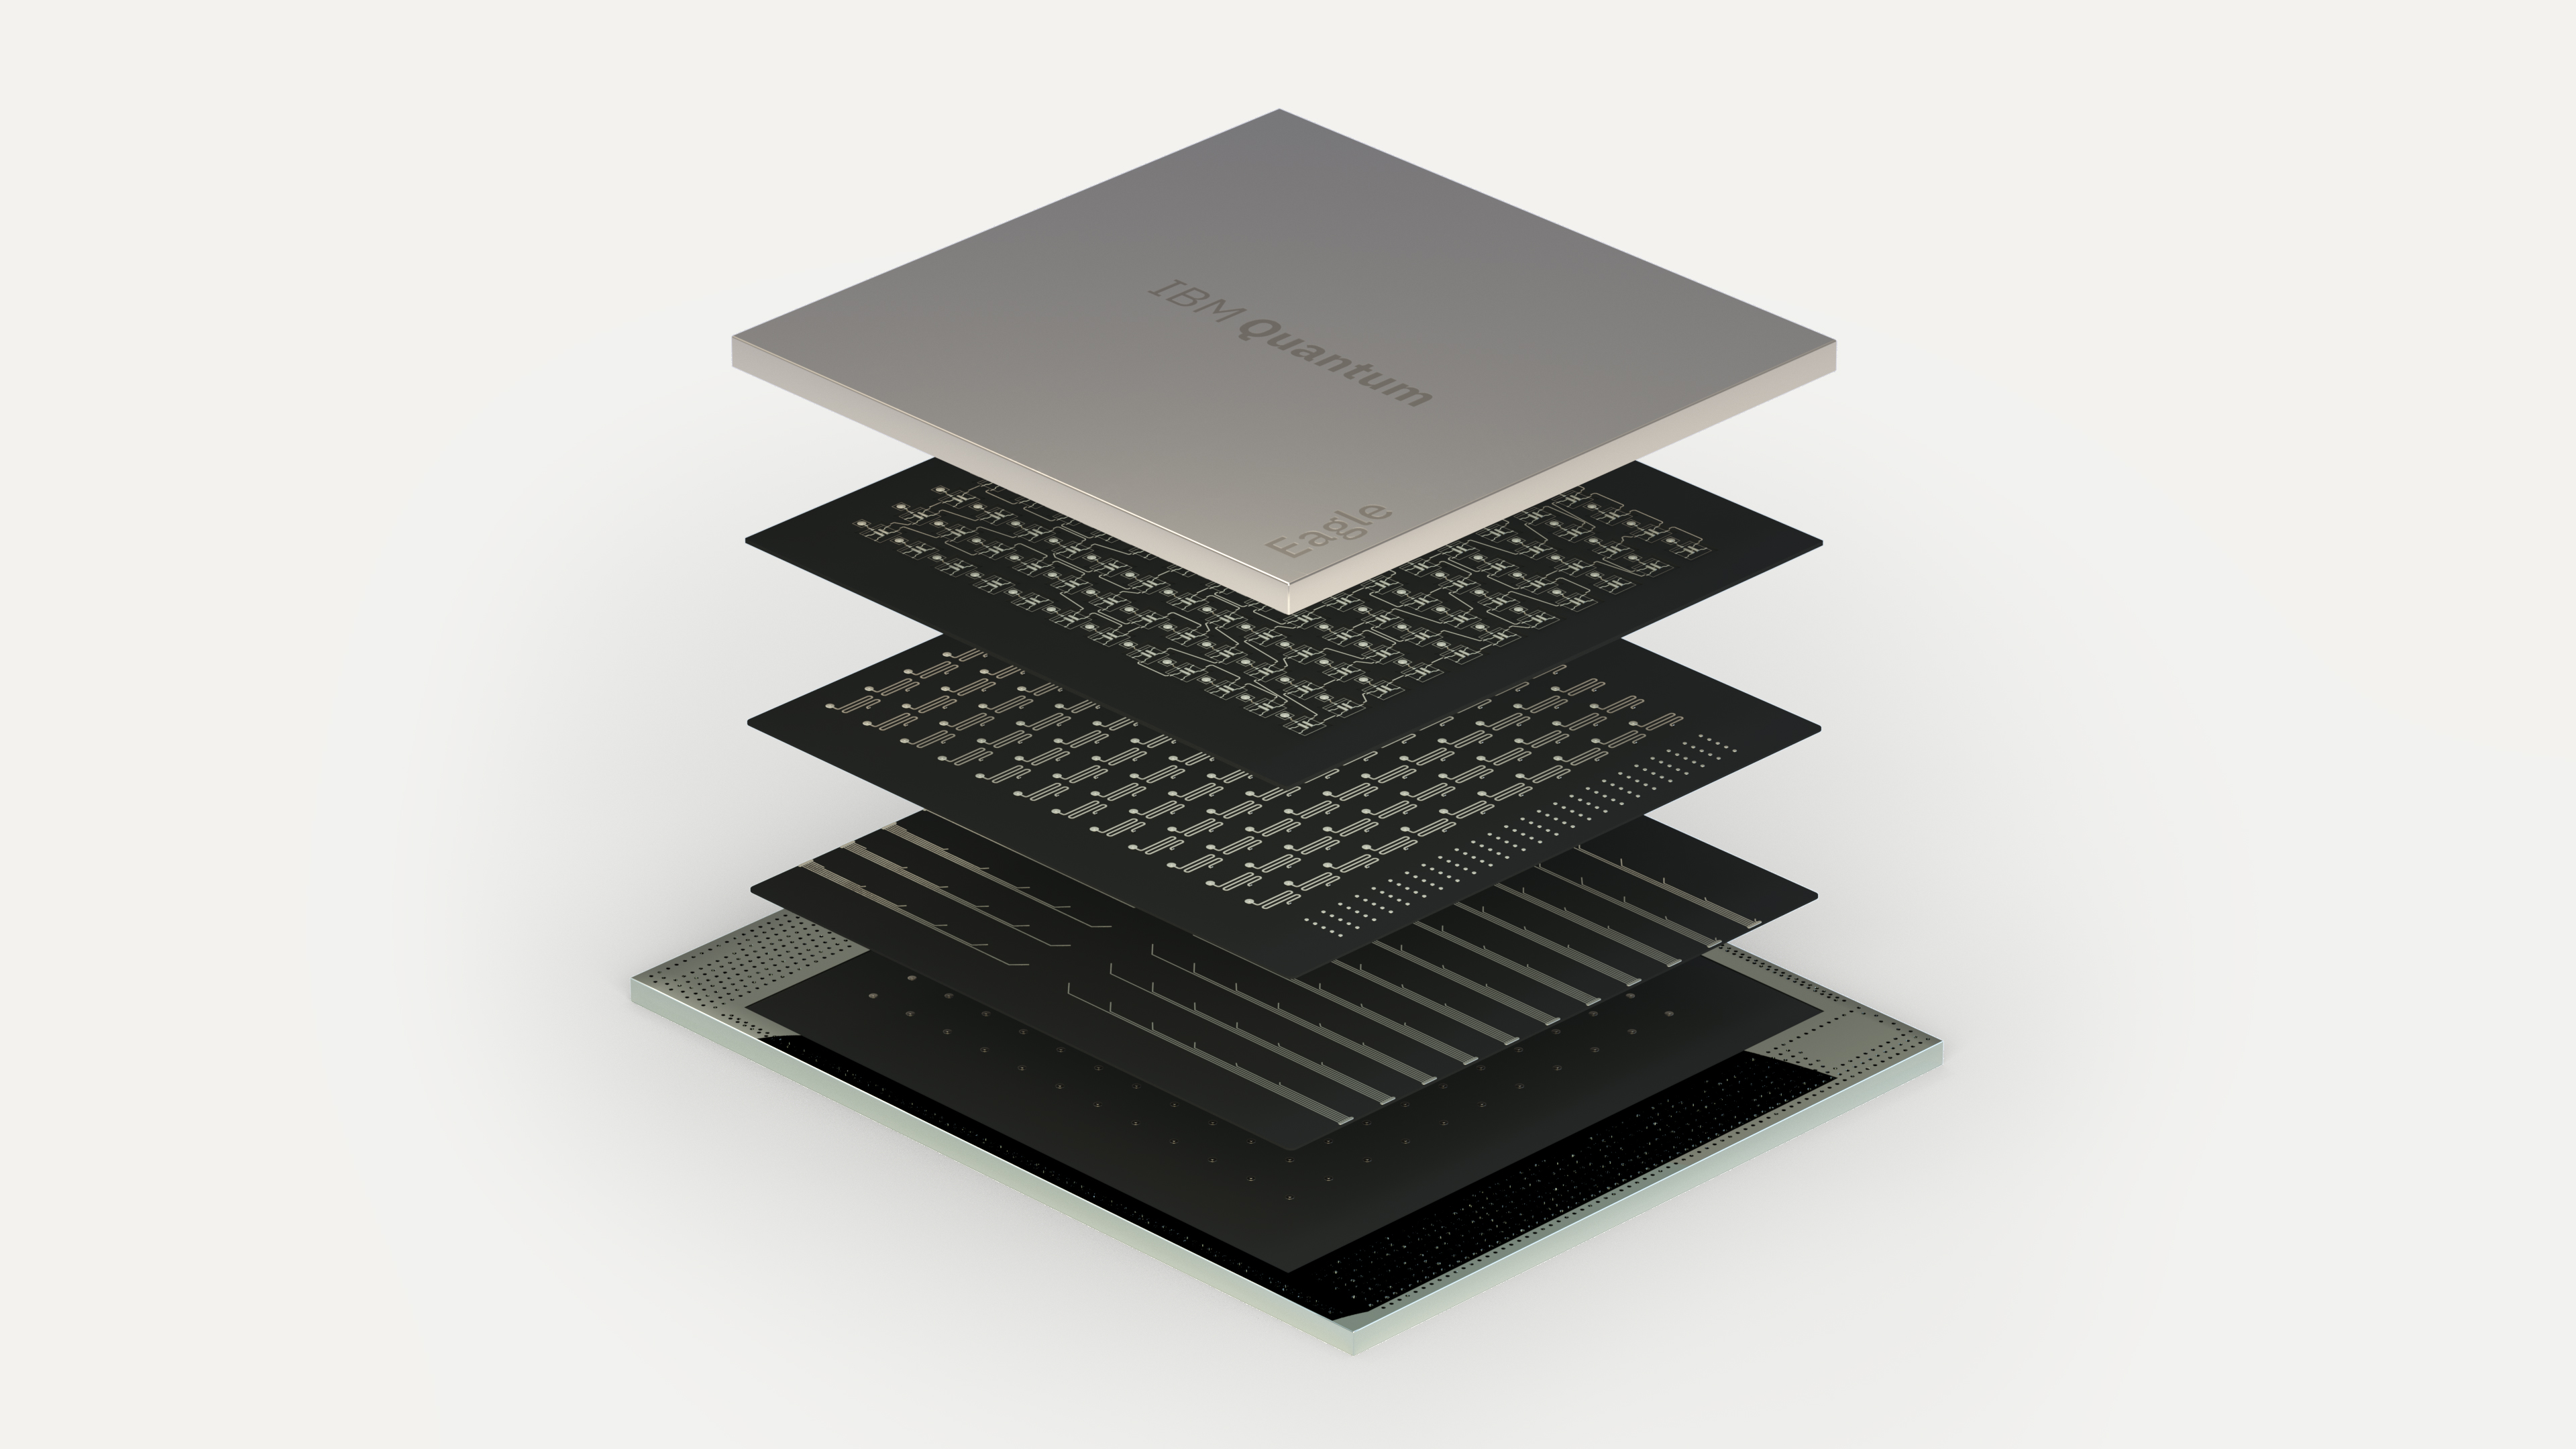
\includegraphics[width=1\textwidth]{relatorio latex/Quantico.jpg}
  \caption{Processador Quântico}
  \label{fig:Quantico}
\end{figure}




\chapter{Conclusões}
\label{chap.conclusao}
Em síntese,  na nossa sociedade atual, os processadores estão presentes em quase todos os dispositivos eletrónicos, tendo sofrido desde os primórdios da sua criação uma evolução contínua no que diz respeito ao seu funcionamento, arquitetura e desempenho. Deste modo, assume um cariz fundamental conhecer as principais aplicações de um processador em função das necessidades de cada utilizador. Neste sentido, destacam-se as \ac{CPU}s associadas quer à \ac{Intel} quer à \ac{AMD} que têm conquistado consumidores com as suas diferentes gamas com destaque para a velocidade. Por conseguinte, foi feito referência à Lei de Moore que demonstra o facto de se poder aumentar o número de transístores, com um custo mínimo e com a mesma quantidade de espaço utilizado. Desta forma, o aumento no número de transístores traduz-se num processador mais rápido e eficiente. Por fim, destacou-se o que o futuro reserva no domínio dos processadores com destaque para a criação de processadores quânticos que serão um dia disponibilizados no mercado, marcando um ponto de viragem na história da evolução dos processadores.

\chapter*{Contribuições dos autores}

O elemento \ac{LL} realizou a pesquisa dos conteúdos abordados no Capítulo 2, no Capítulo 3, no Capítulo 4 e no Capítulo 5, assim como a organização dos mesmos; pesquisa e implementação de: imagens associativas, gráficos; estrutura dos respetivos capítulos; formulação de todo o documento, revisão do relatório final e deteção de eventuais lapsos. 
O elemento \ac{AC} realizou a pesquisa dos conteúdos abordados no Capítulo 2, no Capítulo 3, no Capítulo 6, assim como na organização dos mesmos; pesquisa e implementação de: imagens associativas, bibliografia e acrónimos; estrutura dos respetivos capítulos; formulação de todo o documento, revisão do relatório final e deteção de erros.


\vspace{10pt}
\textbf{Percentagem de contribuição de cada autor:}\\

\autores : 50\%, 50\%\\

%%%%%%%%%%%%%%%%%%%%%%%%%%%%%%%%%
\chapter*{Acrónimos}

\begin{acronym}

 \acro{SSD}{Solid State Drives }

\acro{CISC}{Complex Instruction Set Computers}

\acro{RISC}{Reduced Instruction Set Computer}

\acro{ENIAC}{Electronic Numerical Integrator and Computer}

\acro{PC}{Personal Computer}

\acro{Intel}{Integrated Electronics}

\acro{RAM}{Random Access Memory}

\acro{AMD}{Advanced Micro Devices}

\acro{CPU}{Central Process Unit}

\acro{ISA}{Instruction Set Architecture}

\acro{GPU}{Graphics Processing Unit}

\acro{AC}{António Caetano}

\acro{LL}{Leonardo Luís}  

\end{acronym}

\printbibliography
\end{document}
